\documentclass{beamer}

\usepackage[english]{babel}
\usepackage[UTF8]{ctex}              %lualatex用ctex
% \usepackage[utf8]{inputenc} 

%插入代码
\usepackage{listings}
\usepackage{fontspec}
\setmonofont{Monaco}
\usepackage{xcolor}
% 定义可能使用到的颜色
\definecolor{CPPLight}  {HTML} {686868}
\definecolor{CPPSteel}  {HTML} {888888}
\definecolor{CPPDark}   {HTML} {262626}
\definecolor{CPPBlue}   {HTML} {4172A3}
\definecolor{CPPGreen}  {HTML} {487818}
\definecolor{CPPBrown}  {HTML} {A07040}
\definecolor{CPPRed}    {HTML} {AD4D3A}
\definecolor{CPPViolet} {HTML} {7040A0}
\definecolor{CPPGray}  {HTML} {B8B8B8}
\lstset{
    columns=fixed,       
    frame=none,                                          % 不显示背景边框
    backgroundcolor=\color[RGB]{245,245,244},            % 设定背景颜色
    keywordstyle=\color[RGB]{40,40,255},                 % 设定关键字颜色
    numberstyle=\footnotesize\color{darkgray},           % 设定行号格式
    commentstyle=\it\color[RGB]{0,96,96},                % 设置代码注释的格式
    stringstyle=\rmfamily\slshape\color[RGB]{128,0,0},   % 设置字符串格式
    showstringspaces=false,                              % 不显示字符串中的空格
    language=c++,                                        % 设置语言
    morekeywords={alignas,continute,friend,register,true,alignof,decltype,goto,
    reinterpret_cast,try,asm,defult,if,return,typedef,auto,delete,inline,short,
    typeid,bool,do,int,signed,typename,break,double,long,sizeof,union,case,
    dynamic_cast,mutable,static,unsigned,catch,else,namespace,static_assert,using,
    char,enum,new,static_cast,virtual,char16_t,char32_t,explict,noexcept,struct,
    void,export,nullptr,switch,volatile,class,extern,operator,template,wchar_t,
    const,false,private,this,while,constexpr,float,protected,thread_local,
    const_cast,for,public,throw,std},
    emph={map,set,multimap,multiset,unordered_map,unordered_set,
    unordered_multiset,unordered_multimap,vector,string,list,deque,
    array,stack,forwared_list,iostream,memory,shared_ptr,unique_ptr,
    random,bitset,ostream,istream,cout,cin,endl,move,default_random_engine,
    uniform_int_distribution,iterator,algorithm,functional,bing,numeric,},
    emphstyle=\color{CPPViolet},
    basicstyle=\footnotesize\ttfamily,
}



\usepackage{graphicx} %插入图片的宏包
\usepackage{float} %设置图片浮动位置的宏包
\usepackage{subfigure} %插入多图时用子图显示的宏包



%Theme
% customize your own color and navigation
\usetheme[RGB={12 72 66}]{Simple} % color
\useoutertheme{miniframes}              % navigation
% \usetheme{Berlin}
% \usecolortheme{beaver}
% \usepackage[english]{babel}
\usepackage{fancyhdr}        % header footer
\usepackage{graphicx}        % figure
\usepackage{algorithm2e}
\usepackage{booktabs}
\usepackage{xcolor}
\usepackage{bookmark}




\author{沈宇昊 \\ 210162701031}
\title{Python - 作业2}
\date{\today}
\institute{兰州理工大学}

\AtBeginSection[]
{
  \begin{frame}
    \frametitle{Contents}
    \tableofcontents[currentsection]
  \end{frame}
}

\begin{document}
  % \maketitle

  % \tableofcontents
  

  % title
  % \frame[plain]{\titlepage}
  \begin{frame}[plain]
    \maketitle
    \begin{figure}[htbp] %H为当前位置,!htb为忽略美学标准,htbp为浮动图形
    \centering %图片居中
    
\includegraphics[width=0.3\textheight,height=0.2\textwidth]{new- 2.jpg} %插入图片,[]中设置图片大小,{}中是图片文件名
    % \caption{双叶天下第一可爱} %最终文档中希望显示的图片标题
    % \label{Fig.main2} %用于文内引用的标签
    \end{figure}
  \end{frame}

  % \begin{frame}
  %   \frametitle{Content}
  %   \tableofcontents % 这个命令将会显示目录
  % \end{frame}
  
  \section{第四章}
  \begin{frame}[fragile]
    \frametitle{(1)}
    \begin{figure}[!htb] %H为当前位置,!htb为忽略美学标准,htbp为浮动图形
      % \centering %图片居中
      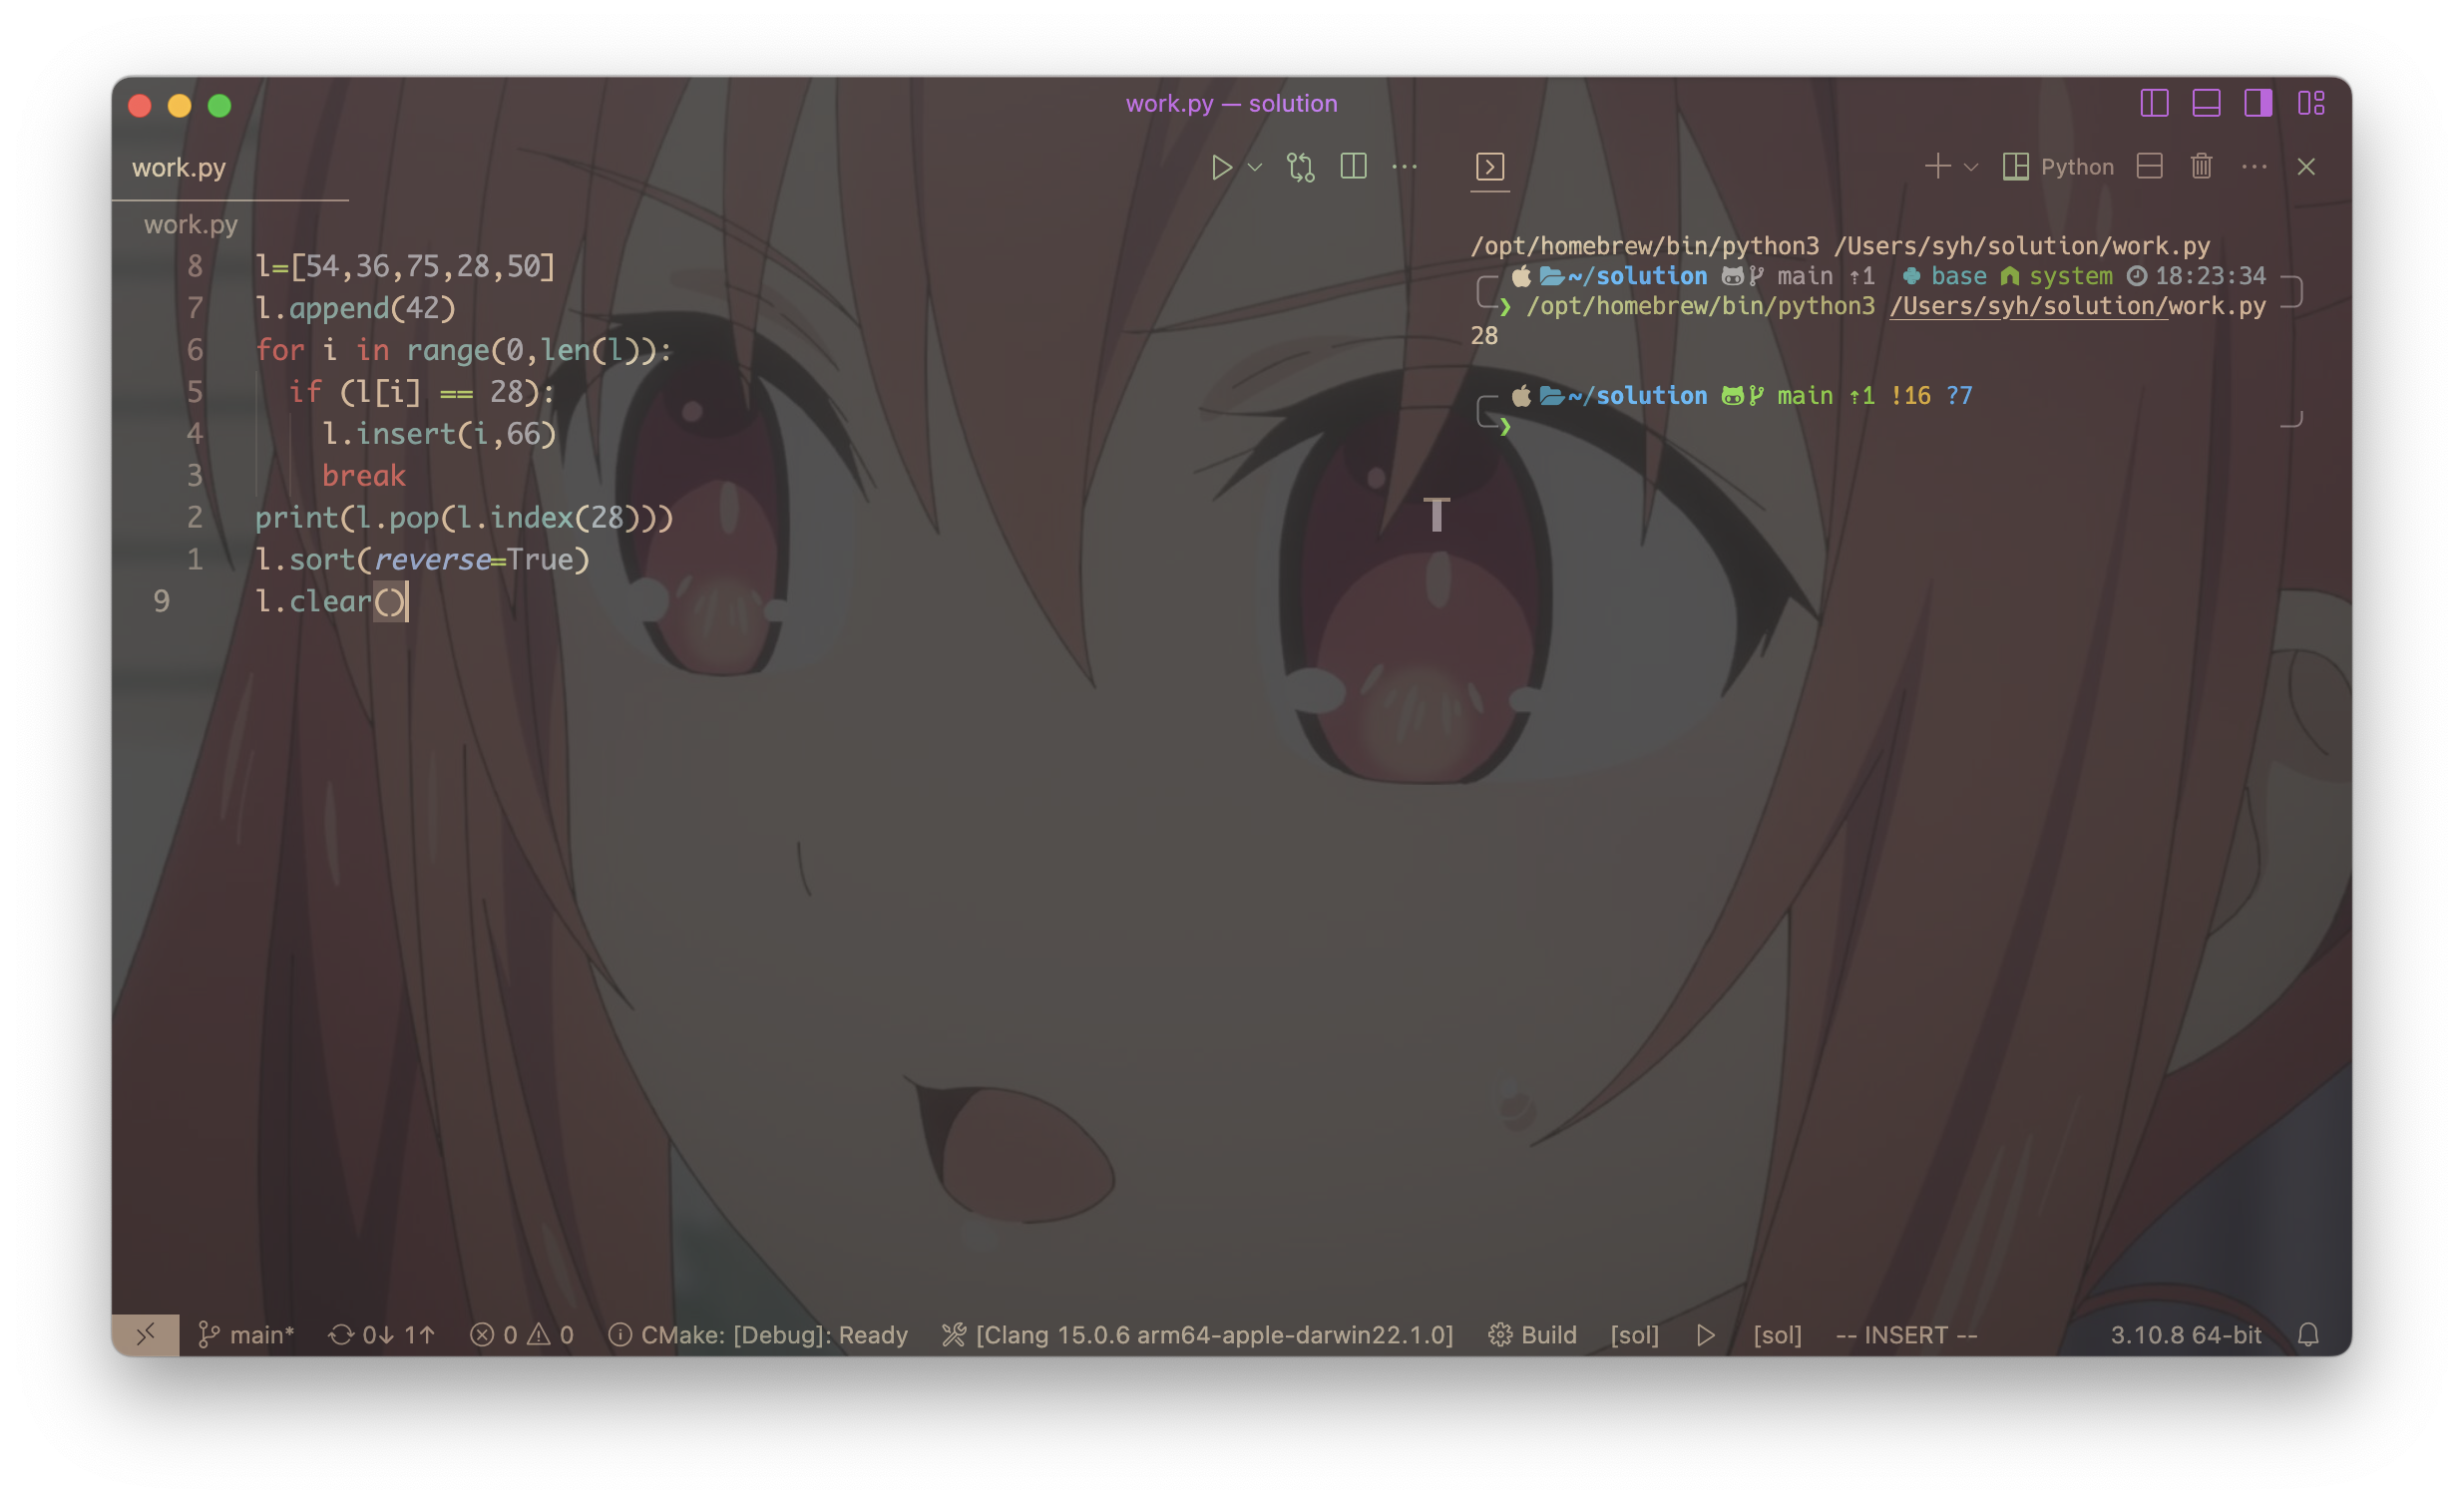
\includegraphics[width=1\textwidth,height=0.8\textheight]{python-4.1.png} %插入图片,[]中设置图片大小,{}中是图片文件名
      % \caption{Main name 2} %最终文档中希望显示的图片标题
      % \label{Fig.main2} %用于文内引用的标签
    \end{figure}
  \end{frame}
  \begin{frame}[fragile]
    \frametitle{(2)}
    \begin{figure}[!htb] %H为当前位置,!htb为忽略美学标准,htbp为浮动图形
      % \centering %图片居中
      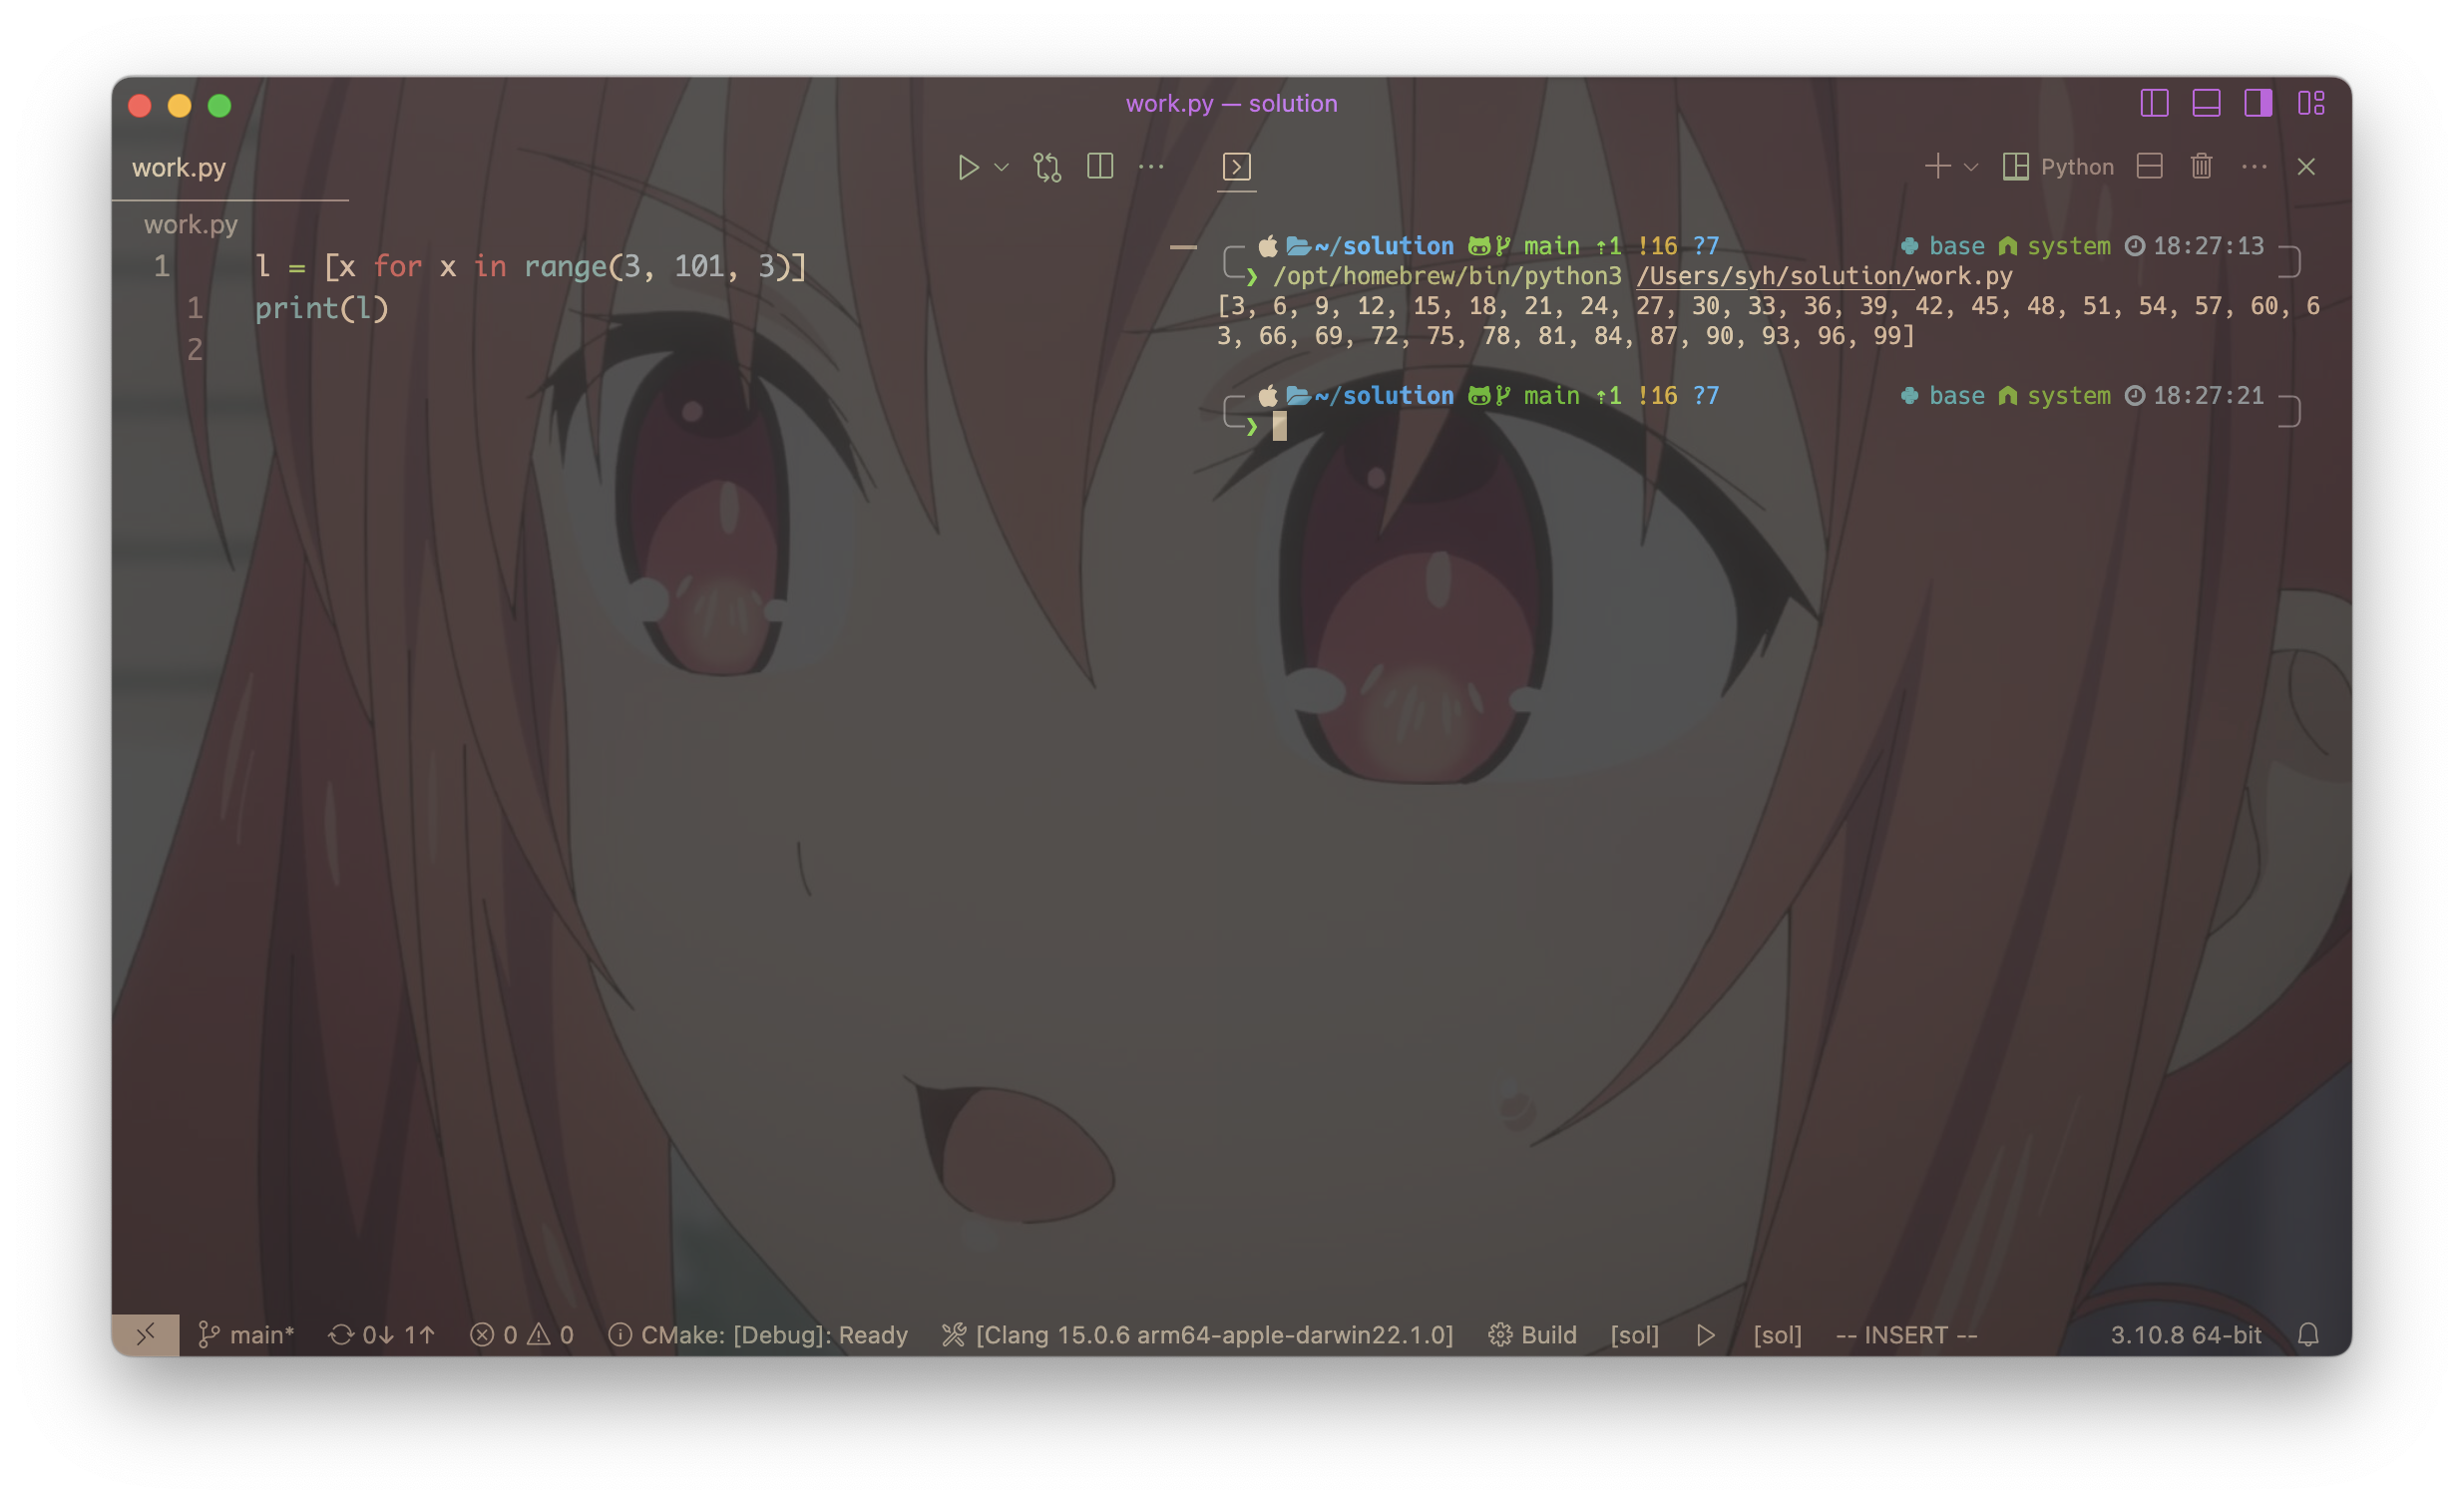
\includegraphics[width=1\textwidth,height=0.8\textheight]{python-4.2.png} %插入图片,[]中设置图片大小,{}中是图片文件名
      % \caption{Main name 2} %最终文档中希望显示的图片标题
      % \label{Fig.main2} %用于文内引用的标签
    \end{figure}
  \end{frame}
  \begin{frame}[fragile]
    \frametitle{(3)}
    \begin{figure}[!htb] %H为当前位置,!htb为忽略美学标准,htbp为浮动图形
      % \centering %图片居中
      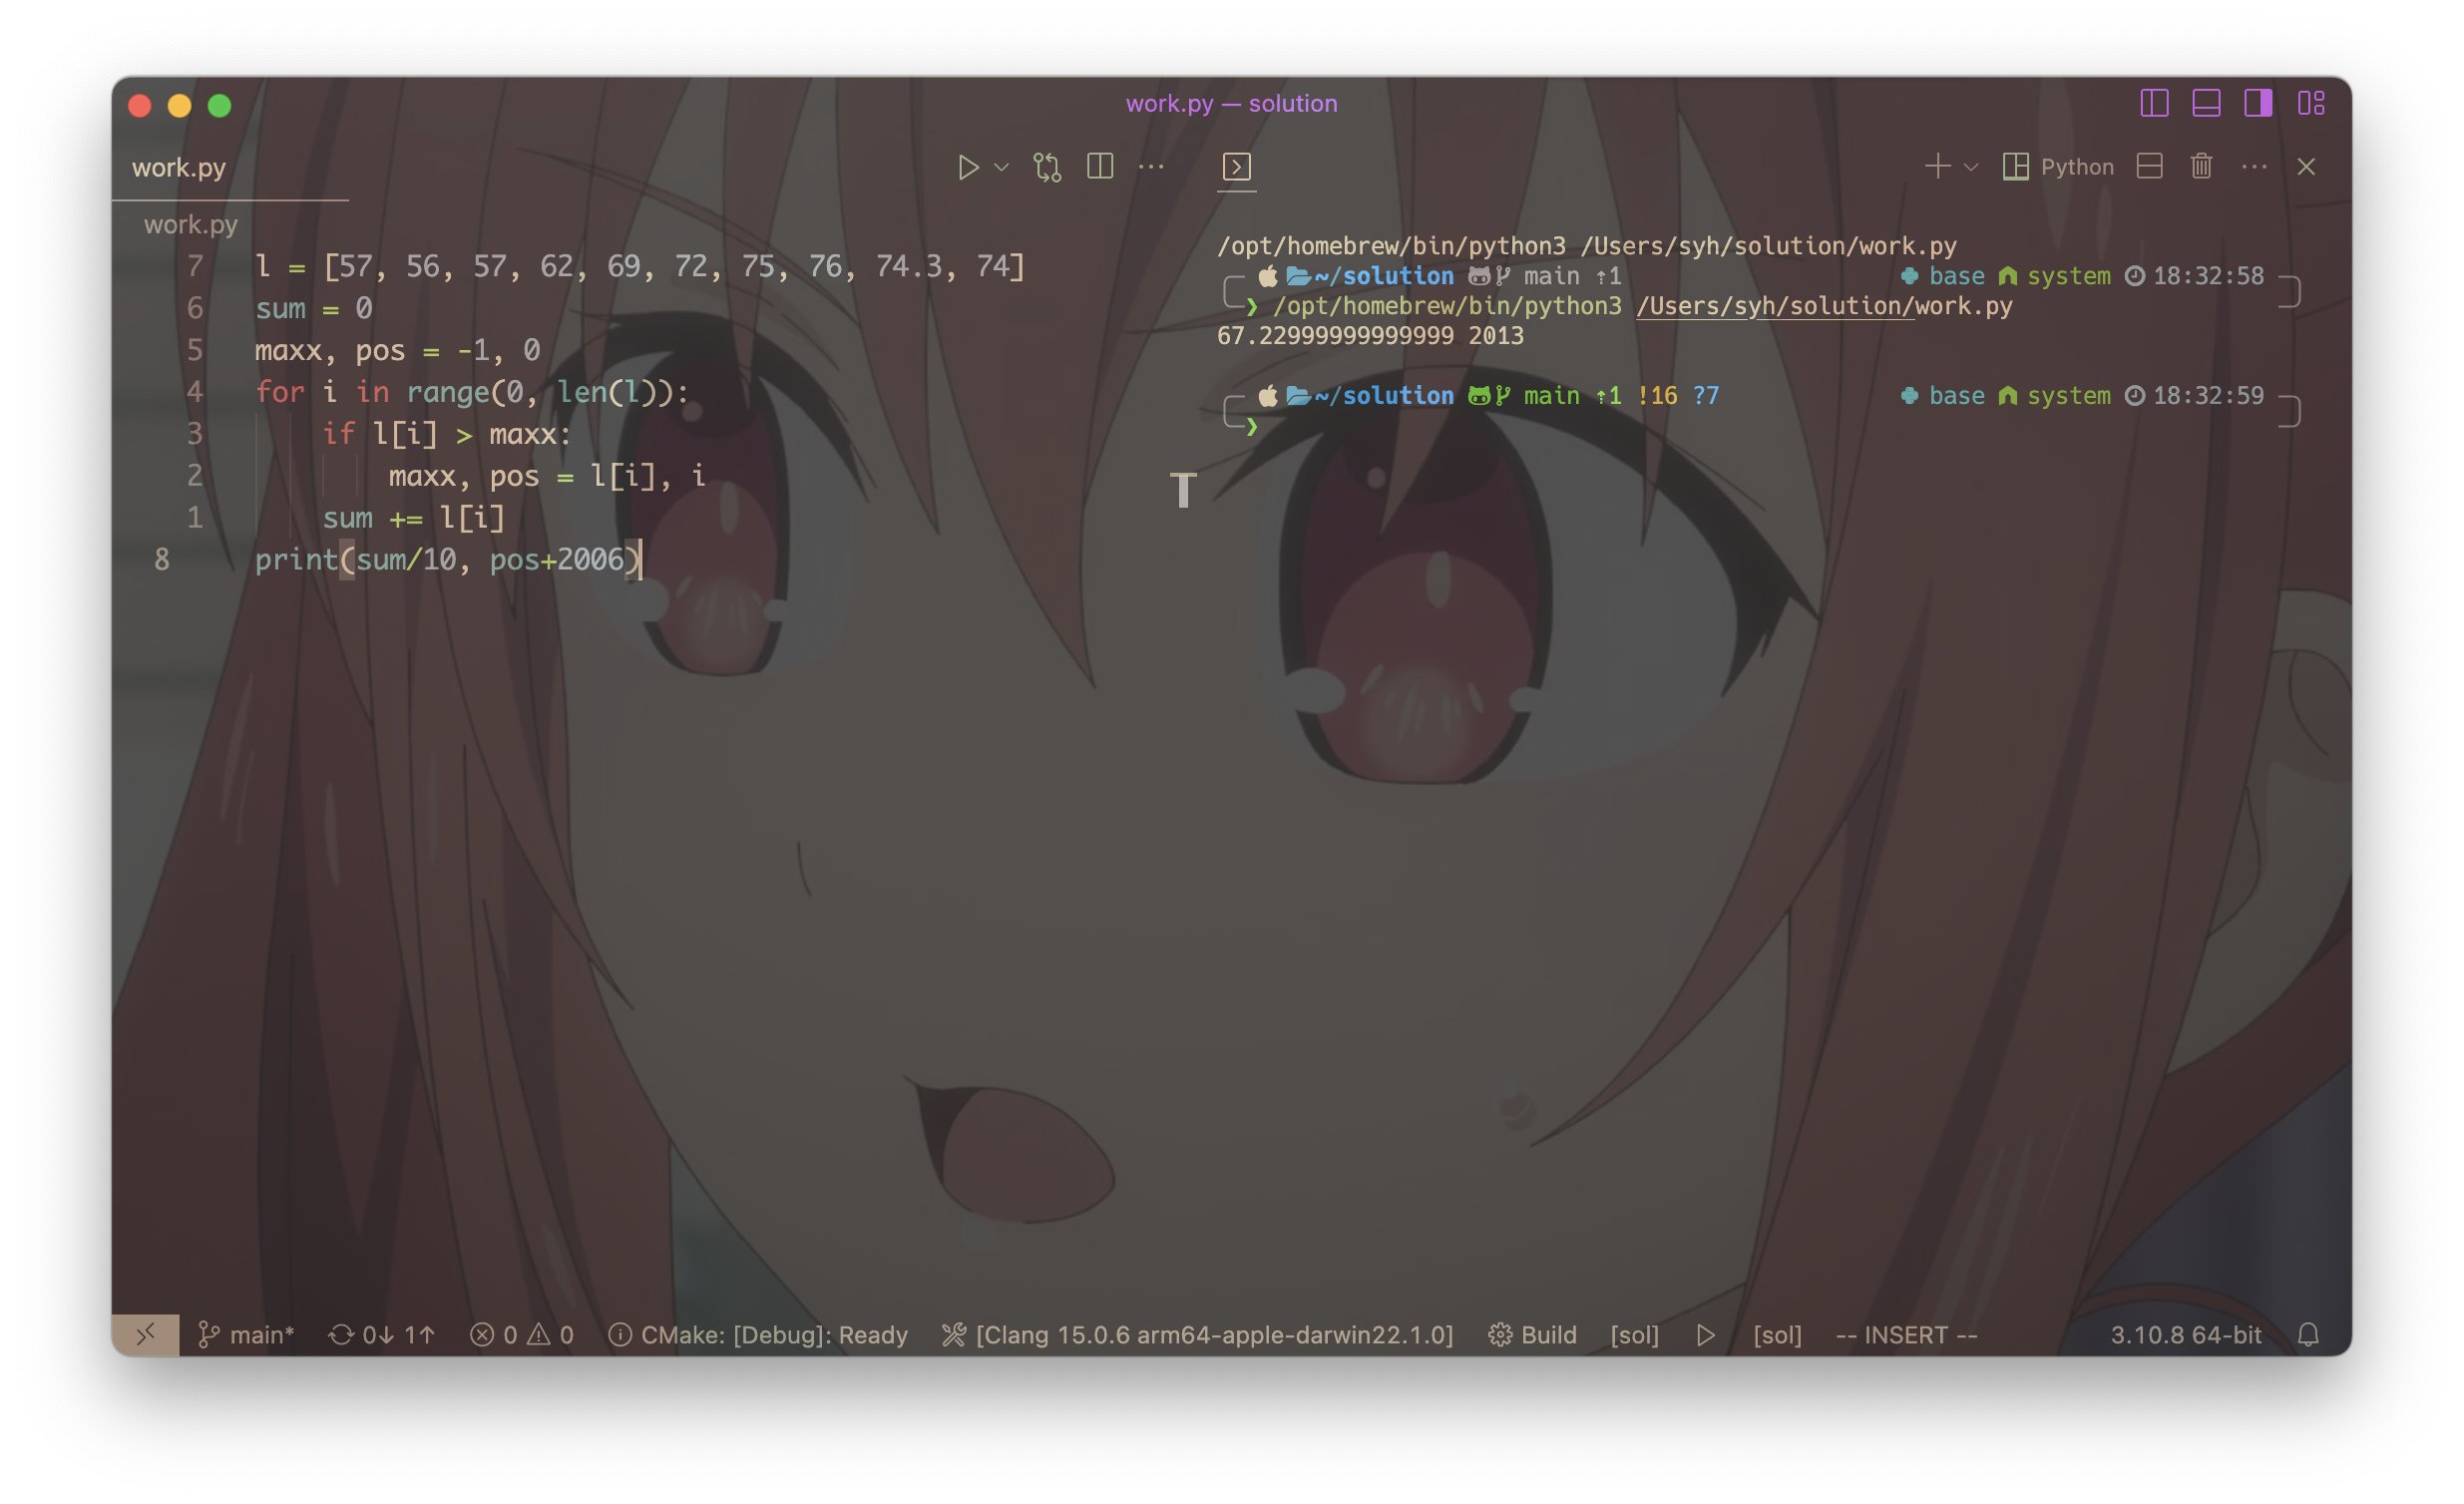
\includegraphics[width=1\textwidth,height=0.8\textheight]{python-4.3.png} %插入图片,[]中设置图片大小,{}中是图片文件名
      % \caption{Main name 2} %最终文档中希望显示的图片标题
      % \label{Fig.main2} %用于文内引用的标签
    \end{figure}
  \end{frame}
  \begin{frame}[fragile]
    \frametitle{(4)}
    \begin{figure}[!htb] %H为当前位置,!htb为忽略美学标准,htbp为浮动图形
      % \centering %图片居中
      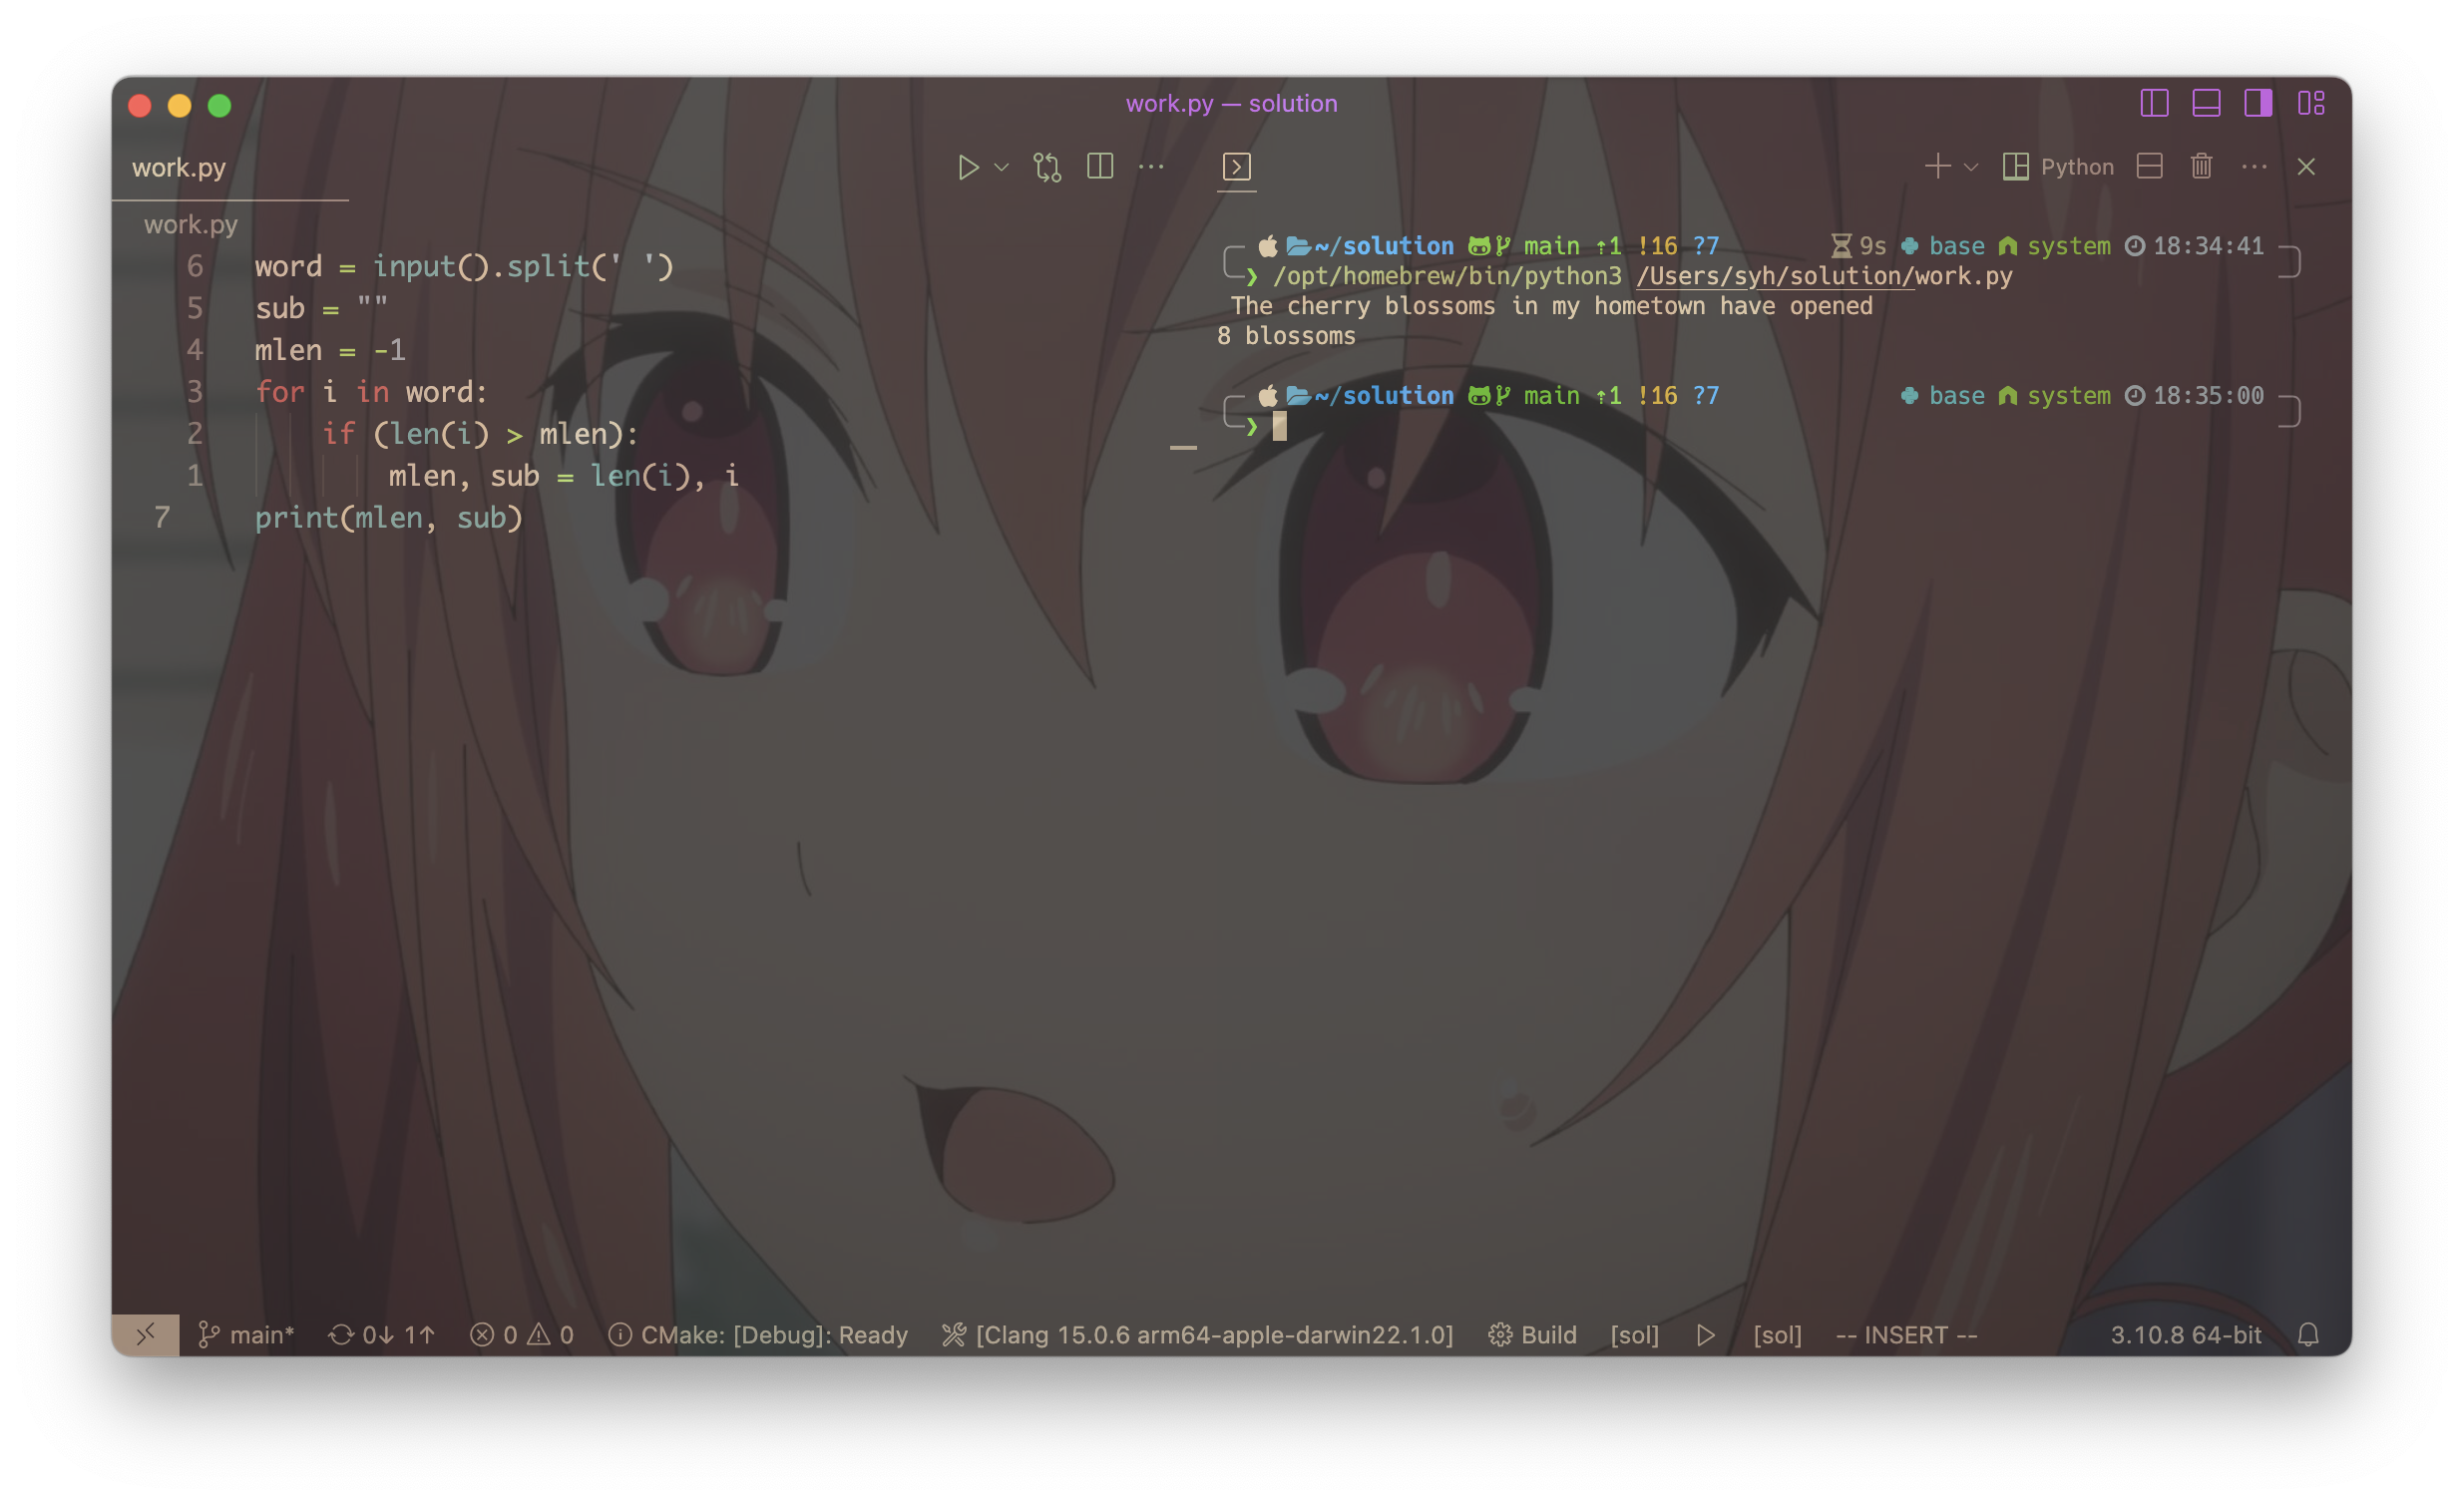
\includegraphics[width=1\textwidth,height=0.8\textheight]{python-4.4.png} %插入图片,[]中设置图片大小,{}中是图片文件名
      % \caption{Main name 2} %最终文档中希望显示的图片标题
      % \label{Fig.main2} %用于文内引用的标签
    \end{figure}
  \end{frame}
  \begin{frame}[fragile]
    \frametitle{(5)}
    \begin{figure}[!htb] %H为当前位置,!htb为忽略美学标准,htbp为浮动图形
      % \centering %图片居中
      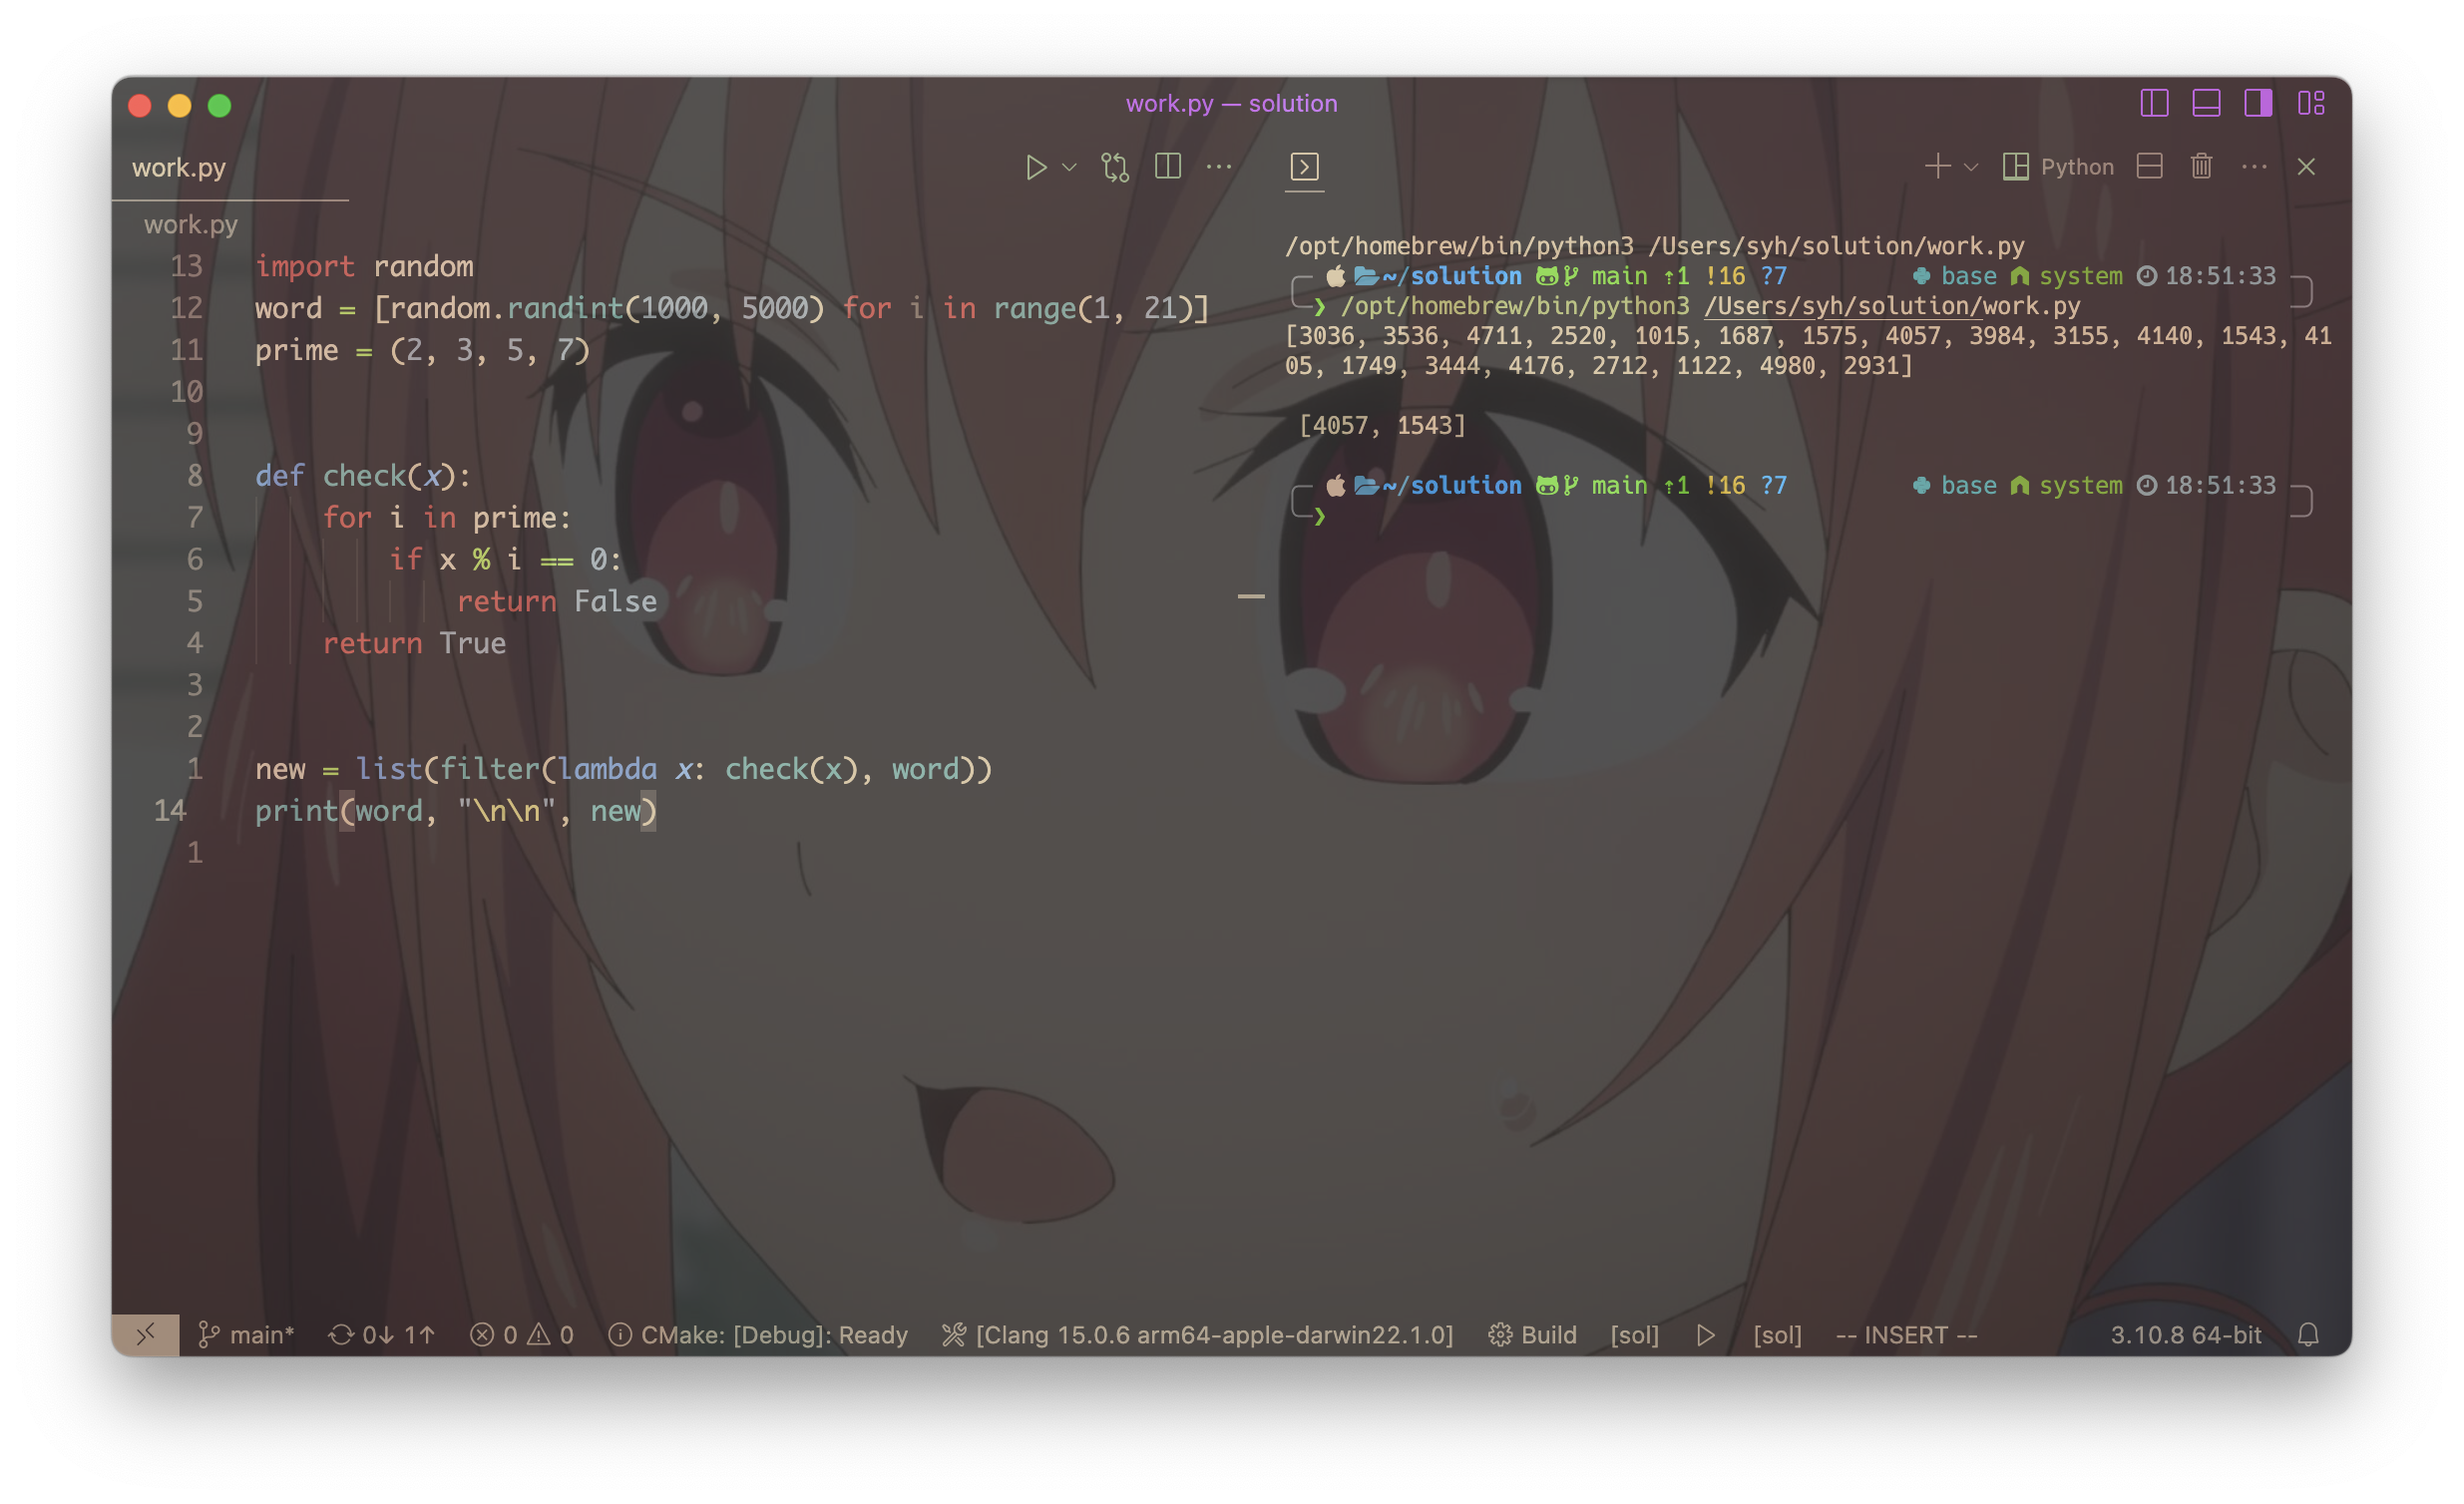
\includegraphics[width=1\textwidth,height=0.8\textheight]{python-4.5.png} %插入图片,[]中设置图片大小,{}中是图片文件名
      % \caption{Main name 2} %最终文档中希望显示的图片标题
      % \label{Fig.main2} %用于文内引用的标签
    \end{figure}
  \end{frame}
  \begin{frame}[fragile]
    \frametitle{(6)}
    \begin{figure}[!htb] %H为当前位置,!htb为忽略美学标准,htbp为浮动图形
      % \centering %图片居中
      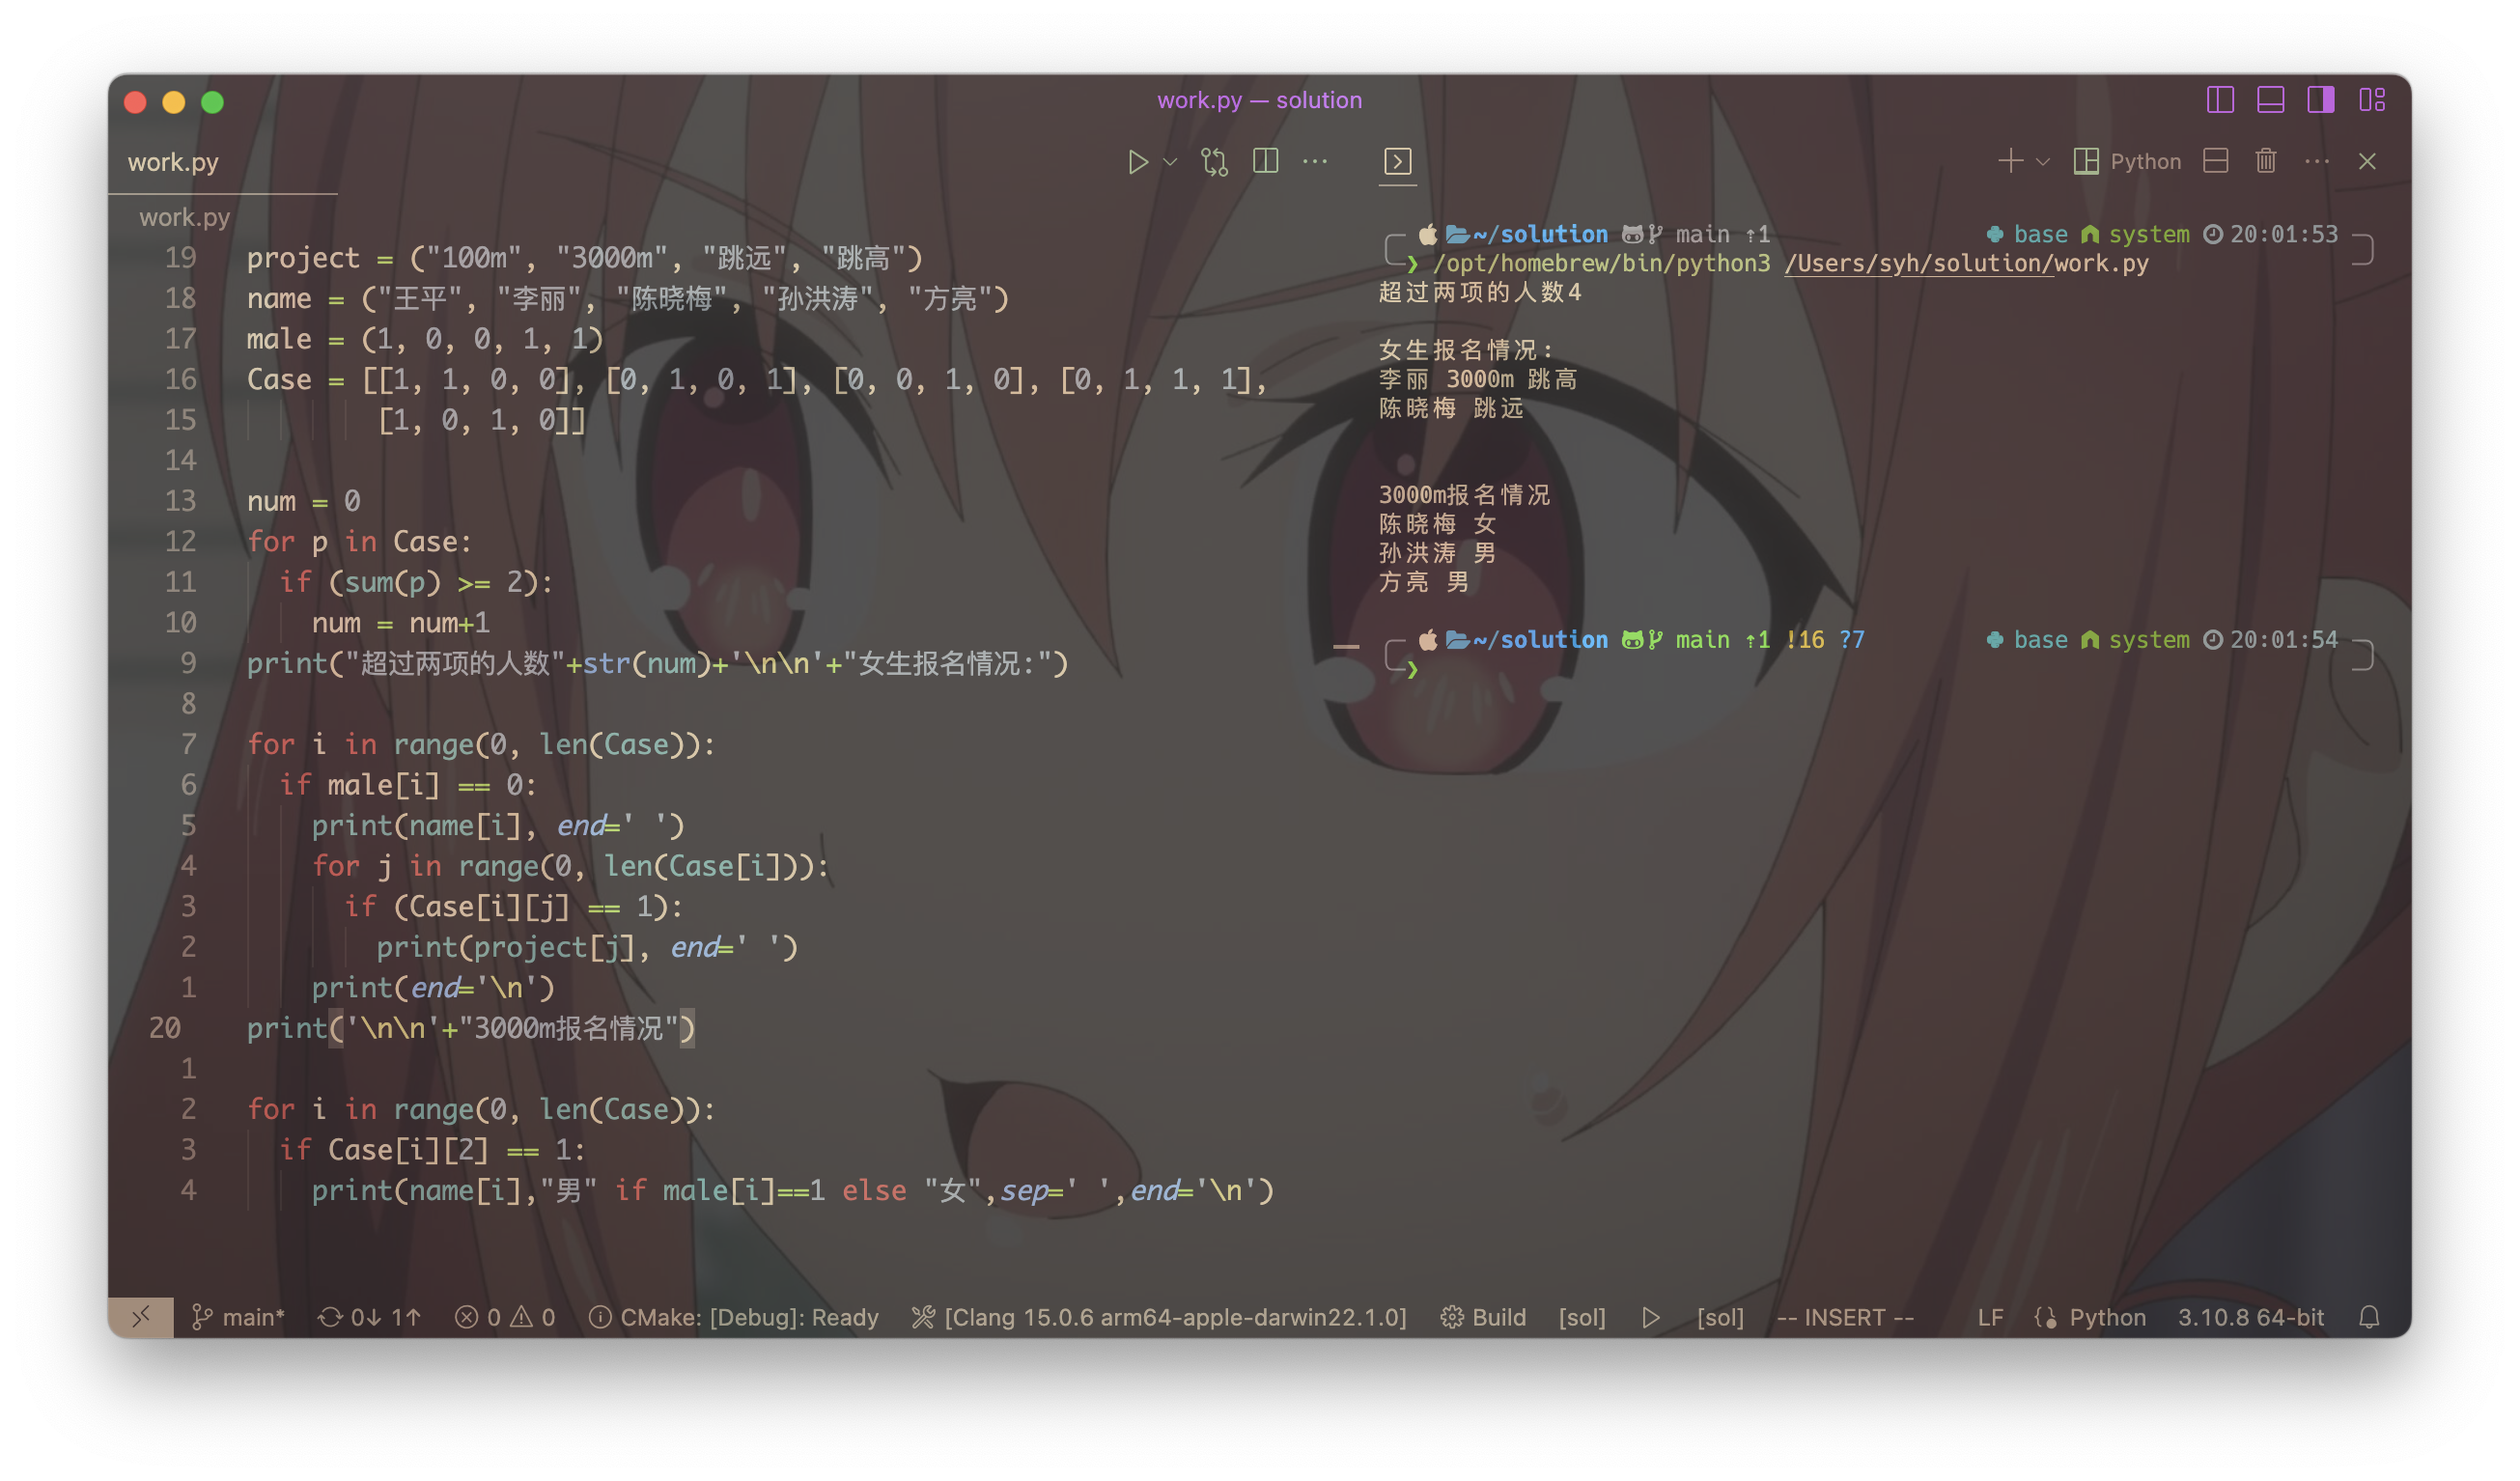
\includegraphics[width=1\textwidth,height=0.8\textheight]{python-4.6.png} %插入图片,[]中设置图片大小,{}中是图片文件名
      % \caption{Main name 2} %最终文档中希望显示的图片标题
      % \label{Fig.main2} %用于文内引用的标签
    \end{figure}
  \end{frame}
\end{document}